\documentclass{beamer}

\usepackage[utf8]{inputenc}
\usepackage{default}
\usepackage{graphicx}
\usepackage{subfig}
\usepackage{rotating}

\usepackage[]{biblatex}
% \bibliography{refs/refs.bib}

% \pdfminorversion=5

%-----------------------------------------------------%
\renewcommand{\d}{\partial}
%-----------------------------------------------------%

\newcommand{\subfigure}{\subfloat}

\usetheme{Warsaw}
\title[Presentation - Kongsberg Defence \& Aerospace]{Diffusion processes in the brain}
\author{Fredrik E. Pettersen}
\date{\today}



\begin{document}

\begin{frame}
\titlepage
\end{frame}



\begin{frame}
 \frametitle{Contents}
 \tableofcontents[hideallsubsections]
\end{frame}

\section{Introduction to neuroscience}
Diffusion processes are extremely important in modern science, and have so many applications that it is challenging to list them all. 
Brownian motion of particles, momentum in liquids, and atomic diffusion are just some examples of processes described by the diffusion equation. \\
\noindent Both in general transport processes, and particularly in diffusion processes, there are cases in which parts of the process cannot be described by a continuum model, but the rest of the process can. 
Examples of such processes are fluid flow in nanoporous media and diffusion in the extracellular space of the brain. There are also many examples in materials design.

\noindent These types of processes can be called multi scale processes in the sense that more than one model is required to describe the entire system. Usually these are on different length scales. 
There are three obvious ways to handle multi scale problems. 
The first alternative is to ignore the problem, and assume that the chosen model can accurately solve the problem. For diffusion processes, this approach often works a lot better than it should. 
A more realistic approach is to create an intermediate scale and model. In the limit between continuum and particle dynamics this is often called a \emph{meso scale} model. 
An example of a meso scale model is dissipative particle dynamics \cite{warren1998dissipative}, where clusters of particles are modeled as individual particles. The particle clusters have different properties than the individual atoms or molecules which make up the substance. 
A final alternative is a \emph{hybrid} model.
Some hybrid models exist today, but these are mostly aimed at specific problems, like dendritc solidification \cite{plapp2000multiscale}, or hybrid fluid flow models which combine molecular dynamics and Navier-Stokes solvers \cite{o1995molecular}. 
Other hybrid solvers for diffusion processes have also been developed \cite{flekkoy2001coupling}, but they are closed in the sense that the computer code is not commonly available. \\

\noindent The aim of this masters thesis is to develop a simple, yet flexible hybrid diffusion solver from the ground and up where all parts of the theory and implementation are fully understood and transparent. 
In principle, any particle dynamics model could be used, but for the sake of verification a stochastic model has been implemented. 
This is no limitation, as the interface to the lower scale model is simple, and the lower scale model works as a standalone unit. \\

\noindent A large emphasis has been put on verification of all parts of the hybrid model. 
Both individually and for the combined, hybrid solver to verify the average behavior of the system.\\

\section{Outline}
\noindent The thesis in your hands has the following structure: \\

\noindent \emph{Chapter \ref{chapter:theory}} contains a detailed review of the coupling between the two models, as well as a look at band diagonal linear systems. \\

\noindent \emph{Chapter \ref{chapter:analysis}} defines the error estimate and shows a thorough analysis of all parts of the developed software in order to verify that it functions properly. \\

\noindent In \emph{chapter \ref{chapter:application}} the developed software is modified to describe a physical application in which a hybrid diffusion solver is demanded. \\

\noindent \emph{Chapter \ref{chapter:results}} presents and discusses the results from the verification of the computer code and the physical application. \\

\noindent Finally, \emph{chapter \ref{chapter:discussion}} discusses the thesis as a whole and looks at possible improvements and extensions that can be done. \\

\noindent The \emph{appendix} is a general guide to debugging the methods that have been implemented during this project.


\section{Diffusion}

\begin{frame}
 \frametitle{Normal diffusion}
 \begin{itemize}
  \item Process of net movement due to a difference in concentration.
  \item Formulated in 1855 by Adolf Fick in the modern way.
  \item Widely used across many diciplines like social studies, economics and biology.
 \end{itemize}

 \begin{equation*}
  \frac{\d C}{\d t} = D\nabla^2C
 \end{equation*}
\begin{figure}[H]
 \centering
 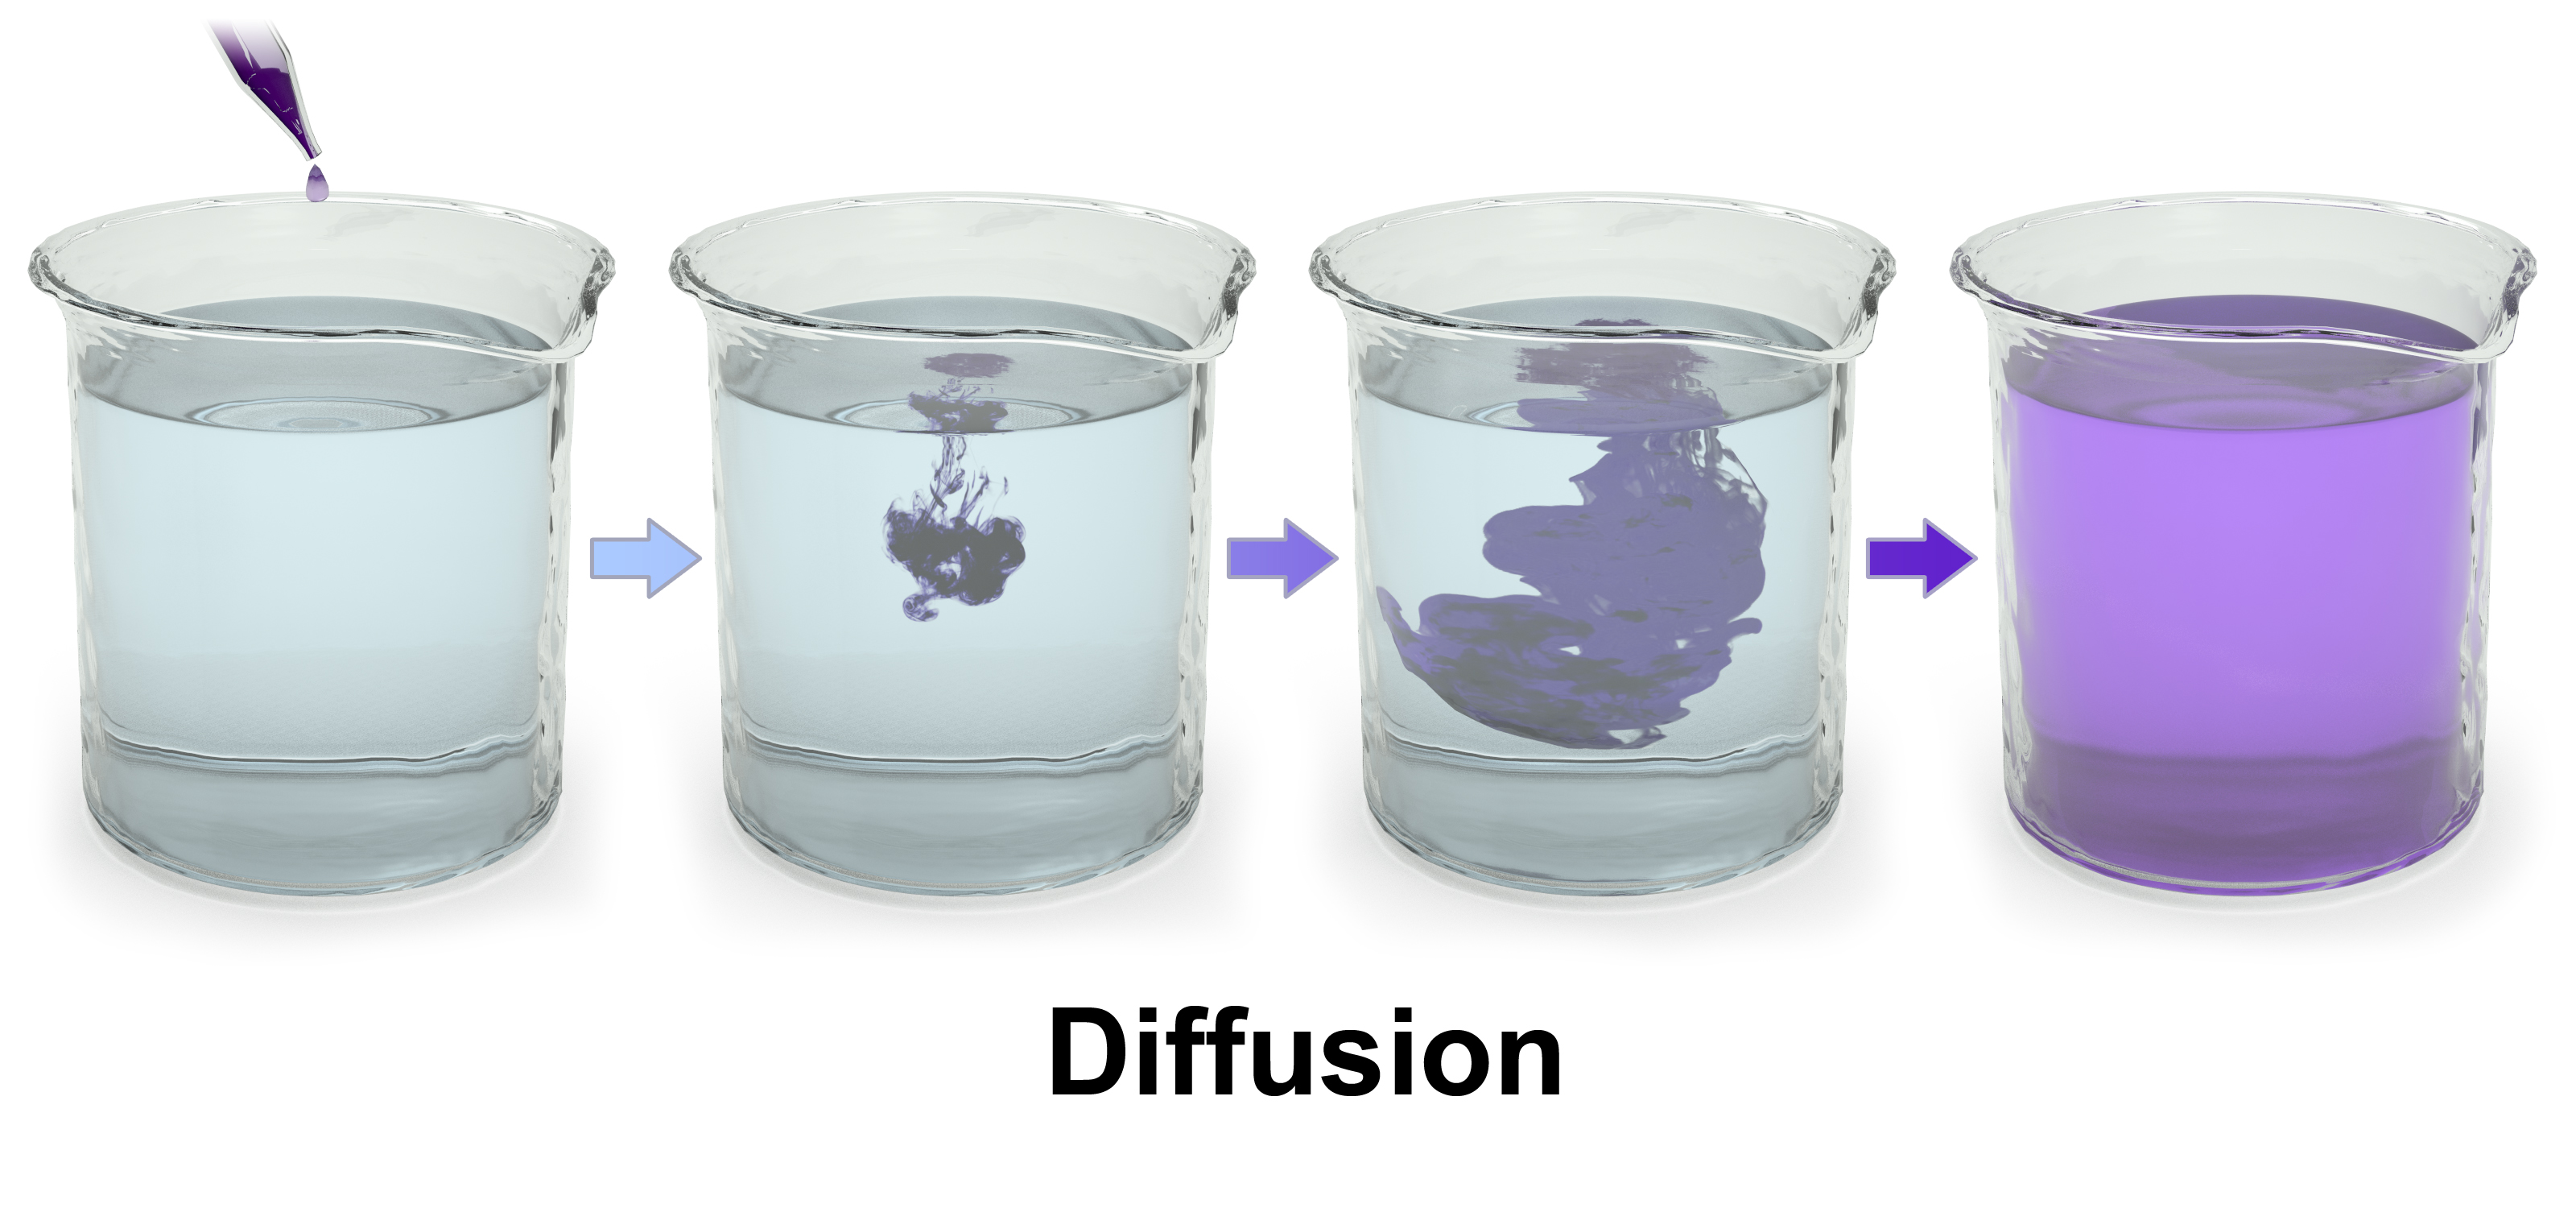
\includegraphics[width=\textwidth]{figures/Diffusion.png}
\end{figure}

\end{frame}



\begin{frame}
 \frametitle{Random walks}
 \begin{columns}
  \column{0.48\textwidth}
  \begin{itemize}
   \item Also widely used in many diciplines.
   \item ``Endless'' possibilities for added complexity.
   \item Conceptually not that difficult.
   \item Recreates diffusion
  \end{itemize}
\column{0.48\textwidth}
\begin{figure}[H]
\centering
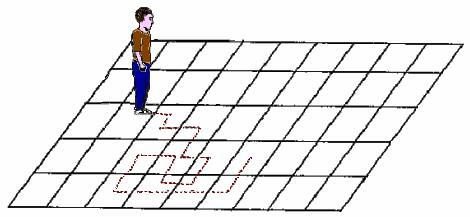
\includegraphics[width=\textwidth]{figures/RW.jpg}
 \end{figure}

 \end{columns}
\end{frame}


\section{Diffusion in the brain}
\begin{frame}
 \frametitle{Diffusion across synapses}
 \begin{columns}
\column{0.48\textwidth}
 \begin{itemize}
 \item Two types of synapses connect neurons - electrical and chemical.
 \item Action potentials triggers release of neurotransmitter into synaptic cleft.
 \item Receiving end passes input on to cell body.
 \item Diffusion across synaptic cleft takes $\sim\mu$s or less.
 \end{itemize}
\column{0.48\textwidth}
\begin{figure}[H]
 \centering
 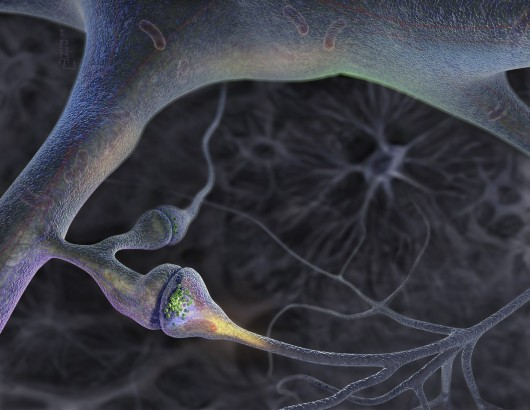
\includegraphics[width=\textwidth]{figures/synapse.jpg}
 \caption{Chemical synapse with dendritic spine.}
\end{figure}
 \end{columns} 
\end{frame}

\begin{frame}
 \frametitle{PKC$\gamma$ diffusion into spines}
 \begin{columns}
  \column{2.0in}
  \begin{itemize}
   \item PKC$\gamma$ is an enzyme associated with learning.
   \item Released from cell body and diffuses through dendrite into spines.
   \item Very low concentrations could require multi scale modeling.
  \end{itemize}
\column{2.0in}
\begin{figure}[H]
\centering
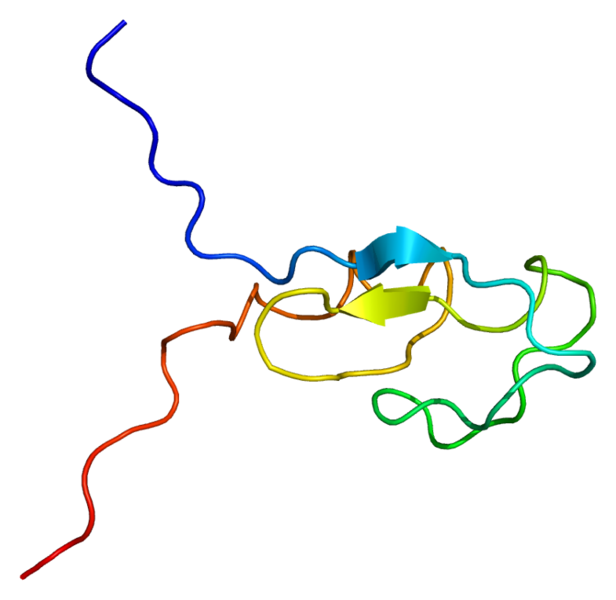
\includegraphics[width=\textwidth]{figures/PKCG.png}
\end{figure}

 \end{columns}

\end{frame}



\begin{frame}
\begin{center}
 \textbf{Thank you!}
\end{center}
% \printbibliography
\end{frame}




\begin{frame}
 \frametitle{My experiment - results}
 \begin{columns}
  \column{2.0in}
  \begin{itemize}
   \item Making spheres of stationary atoms
   \item Measuring self diffusion constant of liquid using Einstein relation
   \item Comparing to self diffusion constant of bulk fluid
   \item Found $\lambda \approx 1.41$
   \item Limitations
  \end{itemize}
\column{2.0in}
% \begin{figure}[H]
% \centering
% \includegraphics[width=\textwidth]{nanoporous_fluid.png}
%  \end{figure}

 \end{columns}

\end{frame}

\begin{frame}
 \frametitle{Random walks}
 \begin{columns}
  \column{2.0in}
  \begin{itemize}
   \item Percolation theory
   \item Random walks and diffusion
   \item Spanning cluster
   \item Results from by Hrab\v{e}tov\'{a} and Nicholson
   \item Limitations
  \end{itemize}
\column{2.0in}
% \begin{figure}[H]
% \centering
% \includegraphics[width=\textwidth]{oppg_a_percmatrix.png}
%  \end{figure}

 \end{columns}
\end{frame}

\section{Some interesting effects}
\begin{frame}
 \frametitle{Firing in auditory nervous system}
%   \begin{columns}
%   \column{2.0in}
  \begin{itemize}
   \item Unanswered questions 
   \begin{itemize}
    \item limitation of tortuosity
    \item tortuosity constant for increasing $\alpha$
   \end{itemize}
   \item Other modeling methods
   \item Multi scale models; the best from both worlds?
  \end{itemize}
% \column{2.0in}
% \begin{figure}[H]
% \centering
% \includegraphics[width=\textwidth]{oppg_a_percmatrix.png}
%  \end{figure}
% 
%  \end{columns}
\end{frame}


\begin{frame}
\frametitle{Output from DTI}
% \begin{figure}
%  \includegraphics[scale=0.3]{contest_logo.jpg}
% \end{figure}
\end{frame}

\begin{frame}
\frametitle{Output from DTI}
\end{frame}

\end{document}